\section{Chapter 5 - Problem (14)}
	A $120 \ g$ hockey puck sent sliding over ice is stopped in $9.7 \ m$ by the frictional force on it from the ice.

	\subsection{Question (a)}

		If its initial speed is $8.2 \ m/s$, what is the frictional force?

		\textbf{R:} \newline

		\begin{figure}[H]
			\begin{center}
				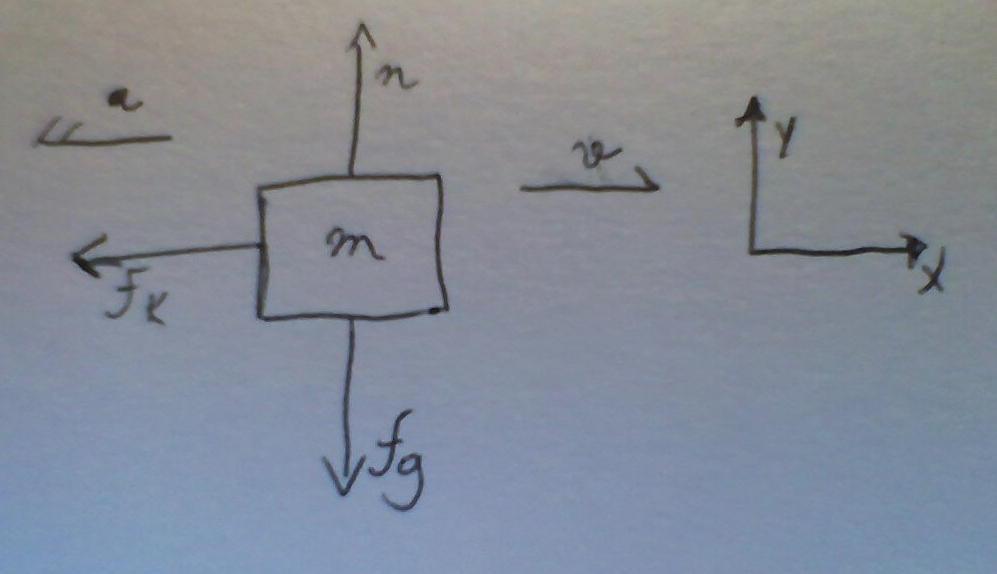
\includegraphics[scale=0.3]{hw6_probleme_fbd}
				\caption{Free-Body Diagram (Problem 14)}
				\label{fig:hw6_probleme_fbd}
			\end{center}
		\end{figure}

		Newton's $2^{nd}$ Law:
		\begin{align}
			\sum F_{x} = \ &ma_{x}& \notag \\
			-f_{k} = \ &m(-a)& \notag \\
			2a(x-x_{0}) = \ &v^{2} - v_{0}^{2}& \notag \\
			a = \ &\frac{v^{2} - v_{0}^{2}}{2(x-x_{0})} = \frac{-v_{0}^{2}}{2x}& \notag \\
			-f_{k} = \ &m\left(-\frac{-v_{0}^{2}}{2x}\right)& \notag \\
			f_{k} = \ &-(120 \ g)\left(\frac{(8.2 \ m/s)^{2}}{2(9.7 \ m)}\right)& \notag \\
			= \ &-(0.120 \ kg)\left(\frac{67.24 \ m^{2}/s^{2}}{19.4 \ m}\right)& \notag \\
			= \ &-0.416 \ N&
		\end{align}

	\subsection{Question (b)}

		What is the coefficient of friction between the puck and the ice?

		\textbf{R:} \newline

		\begin{align}
			f_{k} = \ &\mu_{k}n& \notag
		\end{align}

		Newton's $2^{nd}$ Law to discover $n$:
		\begin{align}
			\sum F_{y} = \ &ma_{y}& \notag \\
			n - f_{g} = \ &m(0)& \notag \\
			n = \ &f_{g}& \notag
		\end{align}

		\begin{align}
			f_{k} = \ &\mu_{k}f_{g}& \notag \\
			\mu_{k} = \ &\frac{0.416 \ N}{(0.120 \ kg)\left( 9.80 \ m/s^{2} \right)}& \notag \\
			= \ &0.354&
		\end{align}
